
\chapter[Renderización de Pan utilizando DVR]{Renderización de Pan utilizando Renderizado Directo de Volúmenes}
Debido a las limitaciones existentes actualmente en el renderizado realista de pan, nos proponemos en este capítulo estudiar la utilización de renderizado directo de volúmenes aplicado a un campo escalar representando la geometría de la miga de pan. Los resultados obtenidos son realistas y se renderizan en tiempo real. La misma evita el uso de estructuras intermedias, simplificando el desarrollo y reduciendo los costos computacionales.

\section{Renderizado Directo de Volúmenes (DVR)}
La técnica de DVR tiene como objetivo crear una representación bidimensional de un volumen
definido por una función de densidad tridimensiopocnal. Para ello, se emiten rayos desde el punto de vista de una cámara en una escena virtual y se utiliza la función de densidad para calcular la cantidad de luz que la cámara recibe en la dirección del rayo. Para esto se evalúa la función de densidad en el camino del rayo y se usan los valores adquiridos para aproximar el efecto de varios fenómenos lumínicos, como pueden ser la extinción, transmitancia, o dispersión lumínica, entre otros. La información obtenida de procesar todos los rayos se utiliza para definir el color de los pixeles en la imagen final.

La radiancia es la cantidad de luz que pasa, o es emitida, desde un punto y atraviesa un determinado ángulo sólido. En el contexto de DVR, el medio que los rayos atraviesan, y que es definido por una función de densidad, es considerado como emisivo. Por lo tanto, cuando se busca calcular la cantidad de luz recibida en la dirección de un rayo, lo que se hace es aproximar la radiancia recibida de un punto distante siguiendo la dirección del rayo. El valor de la radiancia es aproximado como la suma de una radiancia de fondo y la radiancia emitida por el medio por el cuál se mueve el rayo \cite{Kratz2006} :

\begin{equation} \label{eq:general_radiance}  
  L(p_n) = L_b + \int_{p_0}^{p_n} \frac{\partial L(t)}{\partial p} \, dt,
\end{equation}

\noindent donde $L_b$ es la radiancia de fondo, $p_0$ y $p_n$ son los puntos inspeccionados en la dirección del rayo más cercano y más lejano respectivamente, $L(t)$ es la radiancia evaluada en el punto $t$, y $\partial p$ es la distancia entre puntos evaluados. En el momento de calcular $L(p_n)$, la integral es aproximada por una suma.

La extinción es la pérdida de fotones en un haz de luz debido a la absorción en el medio que atraviesa y la dispersión hacia otras direcciones. Algunos de los fotones colisionarán con particulas del medio y serán absorbidas y transformadas en otras formas de energía, mayormente calor. Otras rebotarán y pasarán a moverse en otras direcciones. Estos fenómenos se aproximan usando un coeficiente de absorción para el medio, $k_a$ y un coeficiente de dispersión $k_s$. Si el efecto de dispersión es ignorado, la fórmula que define la cantidad de radiancia absorbida en el largo de un segmento de rayo
es: 

\begin{equation} \label{eq:radiance_absorption}  
    L_b \ e^{- \textstyle  \int_{p_0}^{p_n} k_a(t) \, dt}.
\end{equation}

El valor $\int_{p_i}^{p_j} k_a(t) \, dt$ es llamado coeficiente de absorción y se referenciar\'a como $\tau_{(p_i, p_j)}$.

La transmitancia es un concepto complementario a la extinción y describe la cantidad de luz que pasa por un medio en una dirección determinada. El valor de transmitancia entre dos puntos $p_i$ y $p_j$
es:

\begin{equation} \label{eq:general_radiance}  
  T(p_i,p_j) = e^{- \textstyle \tau_{(p_i, p_j)}}.
\end{equation}

Si la emisión de luz se asume como un término constante ($\rho$) para todos los puntos del medio, la fórmula inicial de radiancia queda:

\begin{equation} \label{eq:ray_radiance}  
  L(p_n) = L_b \ e^{-\tau(p_0, p_n)} + \int_{p_0}^{p_n} \rho \ e^{-\tau(t,p_n)} \, dt.
\end{equation}

Esto significa que la radiancia entre los puntos $p_0$ y $p_n$ se puede calcular como la radiancia de fondo restante luego de la atenuación del medio sumada a la emisión, también atenuada, en todos los puntos del medio que atraviesa el rayo.

La técnica de DVR define un volumen donde una función de densidad se evalúa en intervalos regulares y utiliza esa información para aproximar la transmitancia en esos puntos y de esa manera aproximar la cantidad de luz que llega a la cámara. La suma integral descrita anteriormente se reemplaza por una suma discreta de los puntos evaluados de un rayo donde \'este intersecta al volumen que interesa representar. 

Otros efectos lumínicos pueden ser aproximados. Esto aumenta la fidelidad de la imagen final pero también aumenta el costo de cómputo de la técnica. Algunos de estos efectos son el cálculo de fase, el c\'alculo de luz entrante por dispersión o luz extinguida por dispersión, entre otros. Dado que el objetivo de este trabajo es lograr un renderizado en tiempo real, el algoritmo implementado usa como base el modelo de cálculo de radiancia simplificado que toma en cuenta sólo la
transmitancia del medio.

\section{Implementación}
Se cre\'o un programa de prueba\footnote{disponible en \emph{\url{https://www.github.com/rbaravalle/Pysys}}} para evaluar el sistema de partículas que describe la estructura del pan. Este programa usa un campo escalar representando la miga de pan para generar una textura volumétrica que se interpreta como una función de densidad. Esta textura precomputada se usa como entrada para un motor gráfico que utiliza la técnica de DVR para generar imágenes del pan representado por el sistema de partículas original. Este programa demuestra que el método de renderizado propuesto es compatible con los motores gráficos basados en técnicas de renderización en tiempo real en GPU. Se obtienen imágenes de un material realístico así como efectos de sombras suaves dentro del volumen. Esto significa que las técnicas usadas para renderizar estos materiales pueden ser integradas en cualquier motor de renderizado que soporte shaders.

La malla que utiliza el modelo es un cubo que contiene el volumen definido por el sistema que genera la miga del pan. El código del shader de vértices es muy simple, proveyendo sólamente información geométrica al shader de fragmentos. Este último es donde se encuentra la mayor parte de los cálculos a realizar.

Dentro del shader de fragmentos la primera operaci\'on es calcular la geometría de un rayo cuyo origen es la cámara de la escena y cuya dirección lo lleva hacia el fragmento siendo calculado. Este rayo es recorrido en intervalos regulares, evaluando la textura volumétrica para obtener la densidad del pan en esos puntos. Este valor se utiliza para calcular la transmitancia acumulada desde la cámara hasta el punto evaluado. Una vez que la transmitancia es menor que un valor preestablecido o el rayo sale del cubo que define el volumen, el cómputo termina.

En cada punto evaluado también se computa la transmitancia dentro del volumen desde el punto hacia la fuente de luz en la escena. Esto se hace emitiendo un rayo desde el punto con dirección a la luz y nuevamente calculando la densidad en varios puntos del rayo. Con esta nueva información se aproxima la cantidad de luz que llega directamente al punto considerado, y permite representar sombras dentro del volumen.

La información de transmitancia de los puntos evaluados del rayo principal y desde estos puntos hacia la luz se utilizan para calcular el color final del fragmento. A partir de esta información y tomando diferentes consideraciones artísticas pueden lograrse representaciones realísticas de diferentes materiales. En el caso de las imágenes de muestra presentadas en este trabajo el color del fragmento será más oscuro para areas del volumen que se consideran dentro de la corteza del pan y será de un color amarillo claro para la miga. También se usa un componente especular tenue. La información de transmitancia entre los puntos evaluados y la luz ayuda a proveer detalles de la estructura del pan. La Fig~\ref{fg:fragmentshader} muestra un esquema del cálculo del color final del pixel.

\begin{figure*}[htb!]
  \centerline{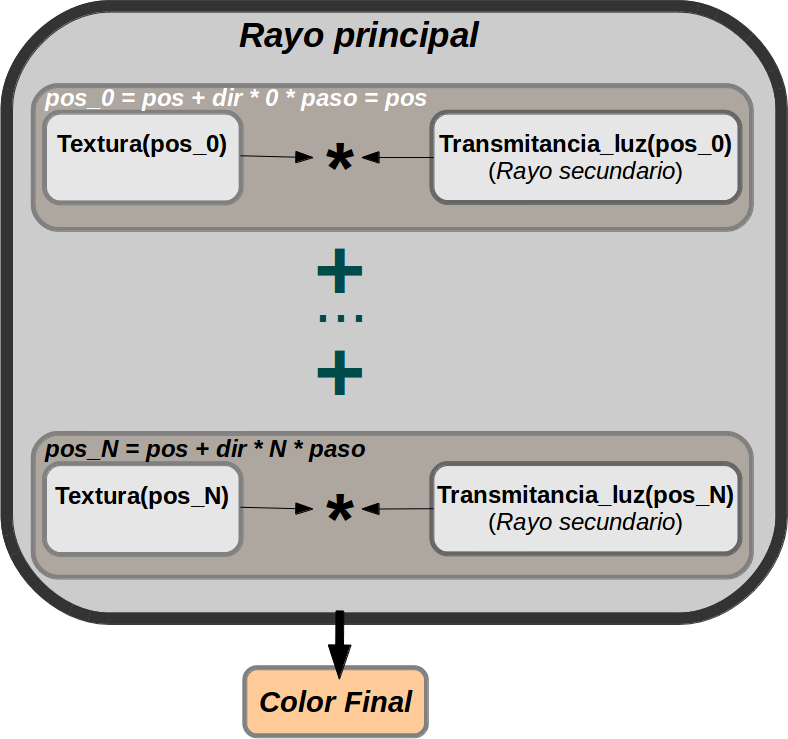
\includegraphics[scale=0.5]{fragmentshader}}
  \caption{Cálculo de color en el shader de fragmentos. }
  \label{fg:fragmentshader}
\end{figure*}


El programa de prueba creado permite modificar parámetros tales como el coeficiente de transmitancia del pan, el límite de transmitancia, el color asignado a la miga y la intensidad de los reflejos especulares, entre otros. Esta capacidad permite crear imágenes que semejan otros
materiales porosos, como por ejemplo esponjas.

\paragraph{Corteza, fetas y cortes}

Las partes del volumen pertenecientes a la corteza y a la miga del pan fueron determinadas manualmente mediante una función que asigna una u otra propiedad a cada punto del volumen a partir de su posición. Por ejemplo, para volúmenes de forma cilíndrica se definió una función que designa como corteza a los puntos que están a más de una distancia predefinida del eje del cilindro.

De la misma manera se define una función que determina si puntos del volumen deben considerarse vacíos, independientemente del valor de la textura volumétrica en ese punto. Esto permite definir fetas de pan de manera sencilla. Un ejemplo del uso de este mecanismo puede apreciarse
en la Fig.~\ref{fg:fig5}.

La asignación de vacío y de corteza deben ser extendidos más allá de ecuaciones basadas en posiciones para poder ser usadas en un proceso artístico.

*MORFOLOGIA MATEMATICA*


En la siguiente sección se presentan y se evalúan los resultados obtenidos.

En esta sección se detallan las imágenes y los tiempos de renderizado obtenidos. 

\subsection{Resultados del renderizado}

Las imágenes obtenidas a partir del método descrito en la sección anterior fueron renderizadas en una computadora con una placa gráfica nVidia GTX 480 ($480$ cores), la cual es normalmente de uso hogareño. La CPU fue una Intel(R) Core(TM) i5-2300 CPU (cuatro procesadores). La resolución de las imágenes es de $1440\times990$ pixels. 
Se obtuvieron diferentes imágenes que semejan materiales horneados. Diferentes tipos de pan pueden ser representados variando los parámetros de transmitancia y colores utilizados (ver Fig.~\ref{fg:fig5}). En la imagen central los patrones producidos por los sistemas de partículas descritos en las secciones previas son claramente visibles. En ese caso, el tiempo de vida de las partículas es diferente para cada una y de esa manera se obtienen burbujas de
diferentes tamaños.

\begin{figure*}[htb!]
  \centerline{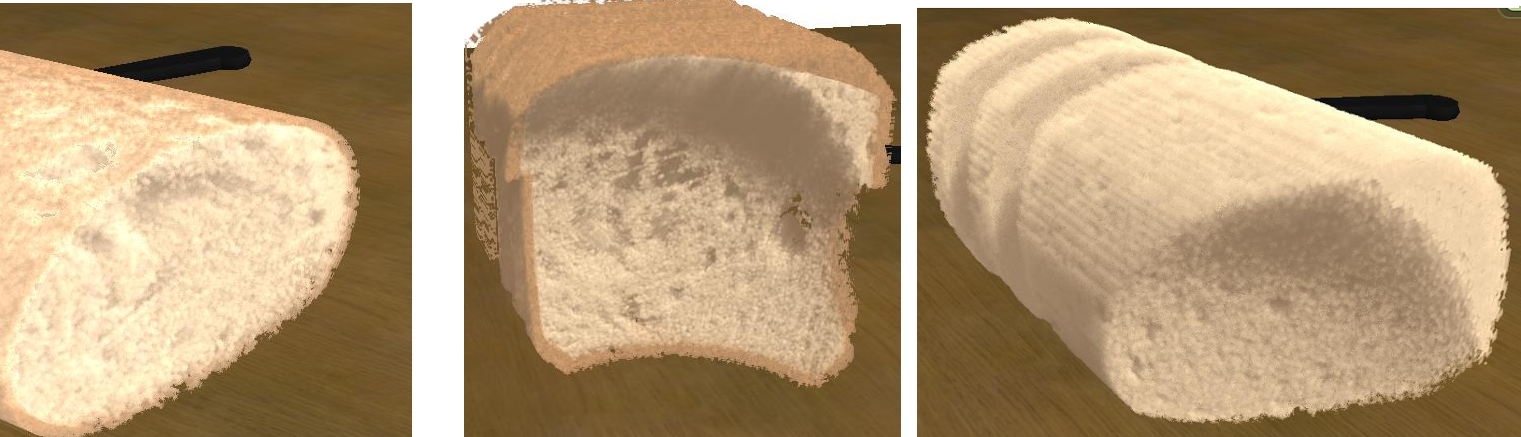
\includegraphics[scale=0.3]{fig5}}
  \caption{Imágenes de diferentes tipos de pan renderizados en tiempo real. La imagen de la derecha muestra un pan sin corteza}
  \label{fg:fig5}
\end{figure*}

Es posible obtener otros materiales (ver Fig.~\ref{fg:fig6}). Estos son el resultado de la variación de parámetros técnicos y artísticos del modelo. En las imágenes de prueba pueden distinguirse un budín (izquierda), un pedazo de torta (medio) y una esponja (derecha). En el caso de la esponja se modificaron los parámetros que definen la función de densidad. Cuando no hay levadura en el proceso de creación puede utilizarse una textura volumétrica cuyos valores provienen de una función aleatoria. La retroiluminación es también aproximada con este modelo (ver Fig.\ref{fg:fig7}). En esa imagen puede apreciarse una esponja retroiluminada junto con la propagación de luz a través del volumen que representa.

\begin{figure*}[htb!]
  \centerline{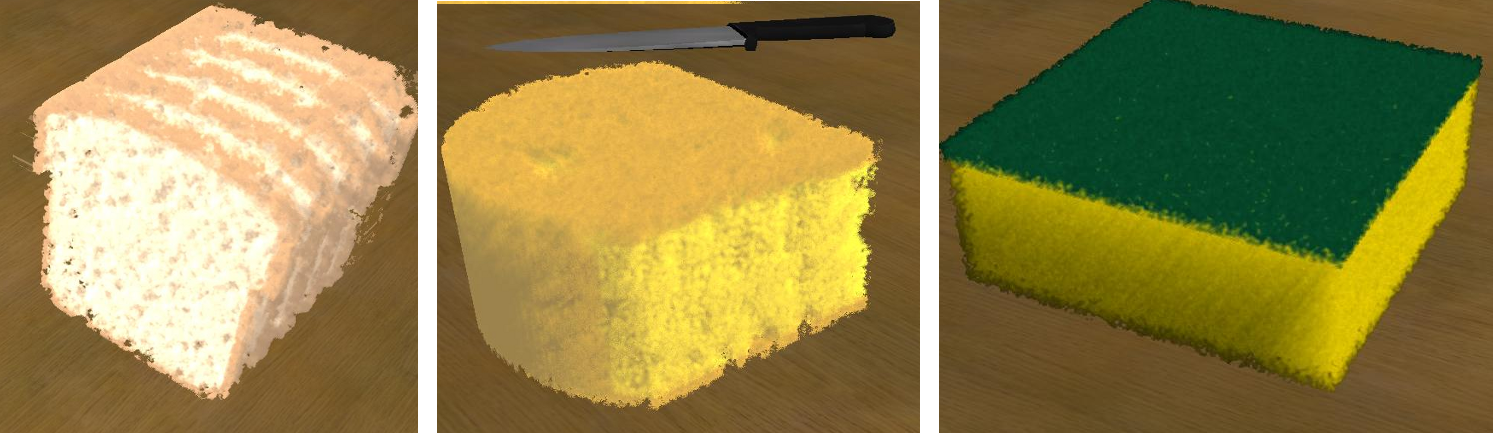
\includegraphics[scale=0.3]{fig6}}
  \caption{Distintos materiales obtenidos a partir de diferentes configuraciones de parámetros. De izquierda a derecha: budín, torta y esponja. }
  \label{fg:fig6}

\end{figure*}

\begin{figure*}[htb!]
  \centerline{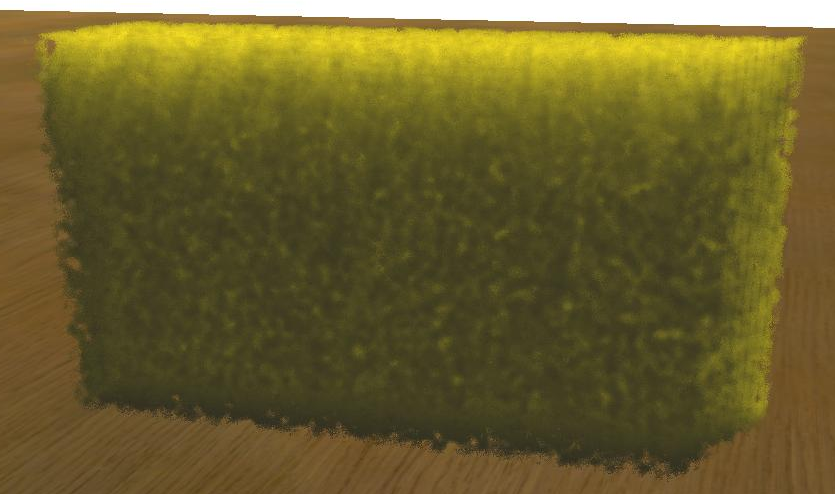
\includegraphics[scale=0.25]{fig7}}
  \caption{Esponja retroiluminada.}
  \label{fg:fig7}
\end{figure*}

\subsection{Tiempos de renderizado}

La mayoría de las imágenes se obtuvieron con tasas de refresco de tiempo real (más de 30 FPS), como muestra la Tabla~\ref{tab:n1}. La eficiencia del proceso se resiente cuando la transmitancia es muy baja (el material es casi transparente), dado que se evaluarán más puntos en los rayos a recorrer antes de llegar al límite de transmitancia. Otro parámetro importante es la distancia entre puntos a evaluar. En la Tabla~\ref{tab:n2} se observa que a medida que la cantidad de rayos y de pasos del rayo aumenta, la velocidad decrece. La tabla muestra que los rayos secundarios constituyen el principal cuello de botella, lo cual es lógico, dado que a cada paso del rayo principal, el mismo computa un rayo secundario hacia la luz.

Experimentalmente se encontró que para todos los casos a evaluar $100$ puntos o más presenta buenos resultados.El proceso escala automáticamente con el número de procesadores en una GPU, por lo cual la tasa de refresco obtenida será mayor en GPUs más rápidas y de más procesadores.


ACTUALIZAR!
\begin{table}[htb]
\centering
\begin{tabular}{|c|c|c|c|c|c|c|}
\hline &  Pan 1 & Pan 2 & Pan 3 & Budín & Torta & Esponja \\
\hline
\hline
 FPS promedio  & 32.2 &  75.5 &  45.2 & 28.5 &  54.2 & 29.7\\
\hline
 Puntos de evaluación &  140 &  140 &  140 & 256 &  140 & 256 \\
\hline
 Transmitancia &  15 &  15 &  15 & 15 &  15 & 2.25 \\
\hline
\end{tabular}
\caption{Tiempos de renderizado y parámetros de las imágenes de prueba.}
\label{tab:n1}
\end{table}

\begin{table}[htb]
\centering
\begin{tabular}{|c|c|c|c|c|c|c|}
\hline
 Pasos del rayo         & 128 &  256 \\
\hline
\hline
 Tiempo total shaders   & 10 ms &  32.5 ms \\
\hline
 Rayo Principal         & 2 ms  & 5 ms  \\
\hline
 Rayos Secundarios      &  8 ms & 27.5 ms  \\
\hline
\end{tabular}
\caption{Detalle de tiempos de renderizado en milisegundos.}
\label{tab:n2}
\end{table}


\subsection{Ambient Occlusion}
Para obtener mayor realismo en las imágenes es necesario aplicar otras técnicas de renderizado. Entre ellas, una muy importante en la apariencia final del pan es la oclusión que produce el ambiente.

*EXPLICACION* 
** PAPER DE OCLUSION

Estas imágenes presentan una aumento notable en el realismo presente en las mismas.

\subsection{Interacción del volumen con el ambiente}
En las imágenes previas se puede observar que el material presenta sombras sobre la mesa que lo sostiene. Para lograr esto, se utiliza una técnica llamada...



\section{Conclusiones}

Según el conocimiento de los autores, éste es el primer intento de llevar a cabo una renderización en tiempo real de pan de manera convincente sin el uso de procesos intermedios complicados (captura de imágenes, generación de mallas, post-procesamiento). Existen buenos resultados de renderizado de pan obtenidos con otros métodos \cite{Cho2007}, pero es difícil comparar ese trabajo con el presentado en este artículo debido a que ni los detalles de la técnica utilizada ni los tiempos de cálculo han sido publicados.

Dentro del volumen a renderizar se pueden definir regiones con diferentes propiedades. Esta idea permite generar imágenes con miga y corteza con diferentes parámetros.

La integración de la técnica descrita con motores gráficos es simple. La información de profundidad de los fragmentos puede obtenerse de manera sencilla y por lo tanto pueden utilizarse técnicas populares de sombras, tales como mapas de sombras.

Los tiempos de cómputo muestran una alta eficiencia del proceso, lo cual depende en gran medida del número de puntos de evaluación usados y la transmitancia del material. Se pueden alcanzcar tiempos de cómputo consistentes con aplicaciones de tiempo real en todos los casos menos en los cuales el volumen ocupa la mayor parte de la imagen a generar, dado que la técnica se calcula casi enteramente en los shader de fragmentos. 

